\documentclass[letterpaper,12pt]{article}

\RequirePackage{GE05}
% this inputs graphicx, too
\RequirePackage{comment}
\RequirePackage[hypertex]{hyperref}
    \hypersetup{colorlinks=true,urlcolor=blue,linkcolor=red}

\def\ClassName{The Global Economy}
\def\Category{Professor David Backus}
\def\HeadName{Group Project \#1}
\newcommand{\phm}{\phantom{--}}
\newcommand{\NX}{\mbox{\it NX\/}}

\begin{document}
\parindent = 0.0in
\parskip = \bigskipamount
\thispagestyle{empty}%
\Head

\centerline{\large \bf \HeadName: Macroeconomic Data} 
\centerline{Revised:  \today}

\medskip
{\it Submit via Blackboard by 9am February 5.}

\begin{enumerate}
\item {\it National Accounts in Beerblastia.} 
Several years ago,
a group of entrepreneurial Stern graduates pooled their resources and
purchased an island in the Caribbean that they named Beerblastia.
After a few years of rapid growth, Beerblastia's economy has begun
to stagnate.  On the principle that there's no good policy without
good data, the head of the government has asked you to serve as
the country's first Chief National Accountant and compile a
set of aggregate statistics for last year.

On your first day on the job, you receive reports of the following
transactions: Local coffee shops sold \$15,000 worth of coffee to
local consumers. To produce the coffee, they purchased \$3,000
worth of coffee beans from local coffee growers. The same growers
also sold coffee for \$5,000 to Starbucks*. (Asterisks denote
foreign companies.) The local textile company bought \$1,000 worth
of wool from an Australian company* and produced \$10,000 worth of
clothes.  Of these clothes, 60\% were sold to domestic consumers,
20\% to the government of Beerblastia, and 20\% to foreigners. The
local textile company also bought 10 Vespas from Piaggio* at
\$1,000 each to use for deliveries. Local fruit producers
harvested \$50,000 worth of bananas. Of these bananas, 60\% were
sold to domestic consumers, 20\% to Chiquita*, and the remainder
to a local subsidiary of Dole*. The subsidiary produced \$20,000
worth of canned bananas, all of which were sold to domestic
consumers. Dole paid \$5,000 in wages to locals and repatriated
the remaining income.  The government raised \$2,000 from
Beerblastians in taxes, paid \$1,000 in pensions to retired
Beerblastians, and purchased 1 Dell* computer (worth \$1,000) to
keep track of its records. Finally, three Beerblastians got short
consulting jobs in the US that paid them \$500 each.

Your mission:  take these reports and construct national accounts.  
Your accounts should include a measure of
GDP;  measures of the expenditure components (consumption,
investment, government purchases of goods and services, and net
exports); and a description of the government's revenues,
expenses, and surplus or deficit.  (35 points)

%\begin{comment}
Answer.  The first step is to compute value-added for each sector
and GDP as the total.  The numbers are:
%?? note coffee now at 15k (from 12k) ****
% summarized in the table,
%\begin{table}[h]
\begin{center}
\begin{tabular}{lcccccc}
\hline\hline%
%\cline{2-7}%
            &  Coffee     & Coffee  &  Textile  &   Fruit   & Canned  \\
            &   Shops     & Growers & Company & Producers & Fruit & Total\\%

\hline\hline%
Sales   &   15,000   & 8,000   & 10,000 & 50,000 & 20,000 
                                                & 100,000\phantom{1} \\%
%\hline%
COGS    &   --3,000  & -    & --1,000   &   -    & --10,000\phm & --14,000\phm \\%
%\hline%
VA          &  12,000     & 8,000     & \phantom{1}9,000  
            & 50,000 & 10,000     & 89,000\\%
\hline\hline%
\end{tabular}
\end{center}
%\end{table}
Here COGS is ``cost of goods sold'' (expenditures on intermediate
products) and VA is value-added.  Total value-added (89,000) equals
GDP.

GDP can also be divided into ``expenditure components,''
consumption, investment, government purchases, and net exports
(exports minus imports). We
find these by tracking sales of final goods to various sectors:
%\begin{table}[h]
\begin{center}
\begin{tabular}{lccccccc}
\hline\hline
Product       & \multicolumn{2}{c}{Private}     & \multicolumn{2}{c}{Government}    & \multicolumn{3}{c}{Net Exports}     \\%
\hline%
              &       C              & I         & C                 & I               & M          & X      & \NX     \\%
\hline\hline%
Coffee        &     15,000           & -         & -                 &    -            & -          & 5,000  & 5,000    \\%
\cline{1-8}%
Bananas       &     30,000           & -         & -                 &    -            & -          & 10,000 & 10,000     \\%
\cline{1-8}%
Canned fruit  &     20,000           & -         & -                 &    -            & -          & -      & -     \\%
\cline{1-8}%
Textiles      &      6,000           & -         & 2,000             &    -            & 1,000      & 2,000  & 1,000      \\%
\cline{1-8}%
Vehicles      &        -             & 10,000    & -                 &    -            & 10,000     & -      & --10,000\phm      \\%
\cline{1-8}%
Computers     &        -             & -         & -                 &   1,000         & 1,000      & -      & --1,000      \\%
\hline\hline%
Total         &     71,000           & 10,000    & 2,000 &   1,000 &
12,000     & 17,000 & 5,000 \\
\hline\hline%
\end{tabular}
\end{center}
%\end{table}
The total is again 89,000, with the understanding that imports $M$
are subtracted.  There are two possible approaches to measuring $I$
and $G$.  One is to define $G$ as total government purchases
(3,000), leaving $I$ as private investment (10,000).  
That's what the US does.  
The other is to define investment as the sum of private and government investment
(11,000), leaving $G$ to mean government consumption (2,000). 
That's what most other countries do.  
Either is ok, as long as you remember what you're doing
and do it consistently.  

The government's budget constraint follows from its revenues and
expenses.  The deficit is the difference: $3,000 + 1,000-2,000=
2,000$.  We'll discuss government accounting later in the course,
but the main contentious issue here is whether to treat government
investment as an expense.  We did, but some official statistics do
not.

%\end{comment}


% --------------------------------------------------------------------

\item {\it Prices and quantities in Darkenbourg.}  
Earlier this month, the
Kingdom of Darkenbourg applied for admission to the European
Union. The ultra-efficient ``Eurocrats'' at the European Commission
returned the application in just three days, arguing that crucial
aggregate statistics were missing. The government has hired you as
a consultant to rectify the omissions. Reviewing the application,
you discover that it reported only GDP at current prices (ie,
nominal GDP) and did not report either real GDP or inflation.

You begin your contract by spending one day a week at the Royal
Office of Statistics teaching the staff about national accounting.
They tell you that Darkenbourg produces only natural cork,
synthetic cork, and running shoes.  They compiled a table that
contains price and quantity data for each of these categories for
1995 and 2005:
\begin{center}
\tabcolsep = 0.12in
\begin{tabular}{lcccccc}
\hline\hline%
     &\multicolumn{2}{c}{Natural Cork}&\multicolumn{2}{c}{Synthetic Cork} &\multicolumn{2}{c}{Running Shoes}\\%
\cline{2-7}%
Year &   Quantity & Price   & Quantity &    Price   &  Quantity & Price    \\
\hline\hline%
1995 &     100    & 12 & 10 & 22 & 80  & 90  \\%
%\hline%
2005 &     110    & 11 & 100 & 7 & 100 & 120 \\%
\hline\hline%
\end{tabular}
\end{center}
Quantities of natural and synthetic cork are measured in thousands
of tons, running shoes in thousands of pairs. Prices are per ton
(for cork) and per pair (for shoes).

Your job is to compute the following statistics from this data so
that Darkenbourg's application can be amended and resubmitted:
%
\begin{enumerate}
\item Nominal GDP, real GDP, and the price deflator for both
years. 
Use 1995 as the base year.  
(20~points)

\item A consumer price index for both years. 
As before, use 1995 as the base year.  (10~points)

\item The annualized rates of inflation over the period 1995-2005
based on the GDP deflator and the CPI, respectively.
Explain briefly why the two measures of inflation are different.  
(5~points)

\end{enumerate}


%\begin{comment}
Answer.
%\begin{enumerate}
The calculations are summarized by:
%** NB:  change of number from 120 to 100....??
\begin{center}
\begin{tabular}{lcccc}
\hline\hline
         &  Nominal GDP  & Real GDP   &  GDP Deflator  & CPI \\
 \hline\hline
1995     &   8,620  & 8,620  &  1.000 &  8,620  \\
2005     &   13,910  &  12,520 & 1.111 & 10,770 \\
Growth (\%)  & 61.37  &  45.24  &  11.1  &  24.94  \\

Annualized (\%) & 4.90 & 3.80 & 1.06 & 2.75 \\
\hline\hline
\end{tabular}
\end{center}
Nominal GDP is the sum of the
product of current prices times current quantities; in 1995, for
example, it equals $12\times 100+22 \times 10+ 90\times 80 =
8,620$.  Real GDP in this table is the sum of 1995 prices times
current quantities; in 2005, it equals $12\times 110+22 \times
100+ 90\times 100 = 12,520$.  (In the jargon of the professionals,
1995 is the base year.) The CPI in this table is the sum of
current prices times 1995 quantities; in 2005, it equals 
$11\times 100+ 7\times 10+ 120\times 80 = 10,770$.


Growth rates are computed this way.  The total growth rate
between 1995 and 2005 is the ratio of the 2005 figure to the 1995
figure, minus one.  Thus the growth rate of nominal GDP is the
solution to
\[
    1 + \gamma \;=\; 13,910/8,620 \;=\; 1.6137 ,
\]
so that $\gamma = 61.37\%$.  The annualized growth rate follows
from compounding growth.  For nominal GDP, the
annualized growth rate solves
\[
    (1 + \gamma)^{10} \;=\; 13,910/8,620
\]
or
\[
    (1 + \gamma) \;=\; (13,910/8,620)^{1/10}
\]
so that $\gamma = 4.90\%$.  Growth rates for other variables are
computed the same way.


Inflation rates are listed above.
Why do the CPI and GDP deflator give different answers?  
Basically they wight the products differently.  
If all prices changed by the same proportion, this wouldn't matter,
but they don't.  In our example, synthetic cork becomes relatively
cheaper than natural cork, and people consume more of it.  The
2005 GDP deflator ``misstates'' its denominator, which is based on
1995 quantities.  The CPI ``misstates'' its numerator, which is
also based on 1995 quantities. As usual, the differences are
modest, but they suggest that there's a limit to the accuracy of
the numbers.  Here the annualized inflation rate ranges from 1.16
to 3.23, and the annualized real growth rate ranges from 1.06 to
2.25.

Another source of possible measurement error in real data 
is quality change in
 products.  The problem doesn't tell us whether or not the
reported prices  take this into account.

%\end{comment}


% ----------------------------------------------------------------------
\item {\it Saving in the US and China.}  
In recent years, China has run a substantial trade surplus (net exports) 
(over 5\% of GDP) and the US a similar deficit.  
The Chinese surplus has become a political issue in the US, 
and implies that China is a net purchaser of foreign assets
as well as a net exporter of goods.    
Using ``Country Data'' from the Economist Intelligence Unit (EIU)
or another source, 
download the expenditure components of GDP (measured at current prices) 
for both countries for the period 1990-present.  Use them to
%
\begin{enumerate}
\item Graph saving, investment, and net exports as ratios to GDP.  
Define saving here as $S = Y - C - G $. 
(15~points) 

\item Comment on the changes in saving and investment rates 
that led to the emerging Chinese surplus and American deficit.  
(10~points) 

\item Speculate on the factors that might have generated these differences 
between the two countries and how they might affect 
trade balances over the next 5-10 years.    
(5~points) 
\end{enumerate}


%\begin{comment}

Answer.  

\begin{enumerate}
\item See the figures.  They're constructed so that net exports
is the difference between saving and investment.  

\item The most striking feature of the figures is that 
both saving and investment are substantially higher in China than the US.
Over the recent past, the saving rate has increased in China, 
and decreased in the US.
Since the trade balance (net exports) is the difference 
between saving and investment, 
the changes in saving rates have led to 
a trade surplus in China and deficit in the US.
Any discussion of the Chinese trade surplus, then, should also address the 
Chinese saving rate:  the two are intertwined.  
  
\item Why would China save so much?  
Good question.
Among the possibilities:  
an aging population saving for retirement and  
an uncertain pension system (leading people to save more to avoid possible
problems), 
maybe even cultural differences.  
Why do Americans save so little?  
One possible reason:  their assets have appreciated, so they 
don't need to save much to have a reasonable ratio of net worth 
to income.  
\end{enumerate}


\begin{figure}
    \centering
    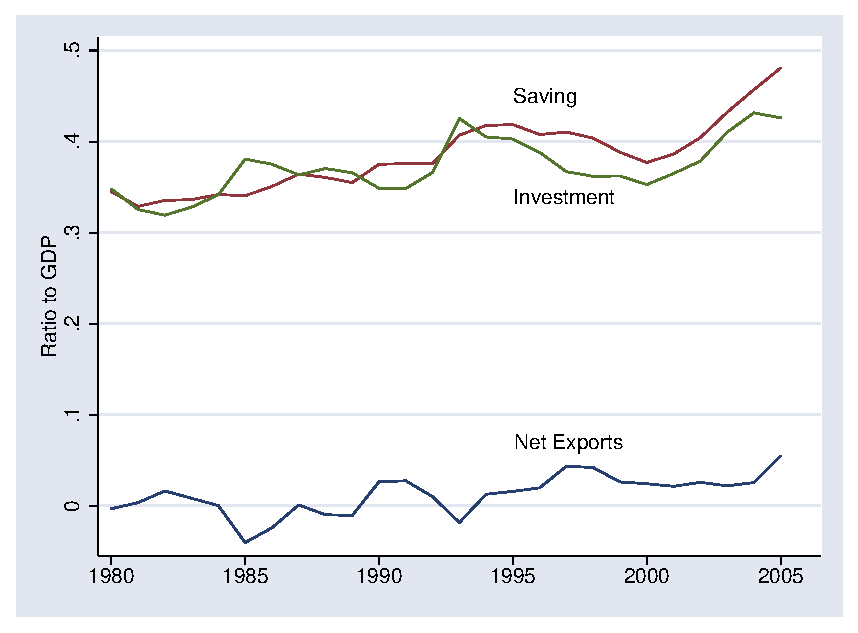
\includegraphics[scale=0.8]{chnflows.eps}
    \caption{Saving and investment in China.}
    \label{fig:chn}%
\end{figure}

\begin{figure}
    \centering
    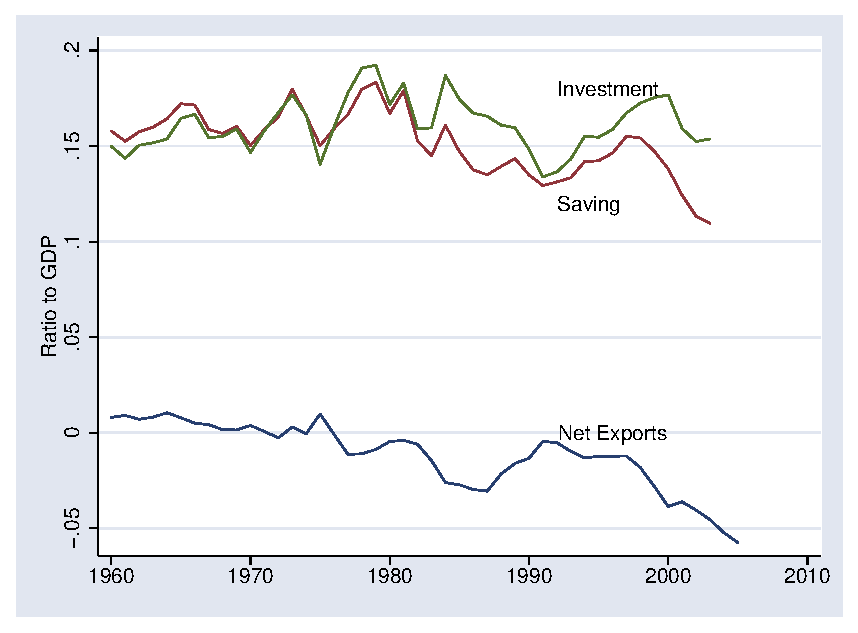
\includegraphics[scale=0.8]{usflows.eps}
    \caption{Saving and investment in the US.}
    \label{fig:us}%
\end{figure}

%\end{comment}

\end{enumerate}


\vfill \centerline{\it \copyright \ \number\year \ 
NYU Stern School of Business}

\end{document} 



% ----------------------------------------------------------------------
\item {\bf The Employment Situation.} The most closely followed
number on Wall Street is nonfarm payroll employment, an estimate
of the number of people working (``jobs'') computed from a survey
of firms. This and other employment data are reported by the
Bureau of Labor Statistics in its monthly report, {\it The
Employment Situation\/}.  The January number will be released at
8:30am (ET) on February 4.

Every month,  the BLS (as it's called) conducts a survey of
payroll records known as the Current Employment Statistics (CES)
or payroll survey.  It covers more than 300,000 businesses and is
used to construct aggregate and industry data on employment, hours
worked, and earnings of workers on nonfarm payrolls for the entire
US.  A similar survey collects data from households.

Your mission is to ``forecast'' the change in nonfarm employment
from the payroll survey between December and January.  You will be
given a spreadsheet (see Blackboard) reporting nonfarm employment
over the last few years. The spreadsheet contains two series; one
is seasonally adjusted, the other is not.  The most recent numbers
are preliminary.

Use this data to:
%
\begin{enumerate}
\item  Comment on the most likely sources of seasonal variation in
employment.  (10~points)

\item Speculate on why the seasonally adjusted series still
appears so erratic. (10 points)

\item Propose an estimate for the change in nonfarm employment
between December and January.  Comment briefly on the reasons for
your estimate.  (10 points)

\end{enumerate}


Answer. The exercise illustrates two issues:  seasonality and
``noise.''  Employment data (like lots of macroeconomic data) has
a strong seasonal, and month-to-month changes are erratic enough
to suggest either that the world is erratic or that there is
measurement error in the data.  Either way, the month-to-month
changes need to be adjusted to give a reliable reading of the
growth of the economy over (say) a year or more.
%
\begin{enumerate}

\item Seasonality.  You might imagine -- especially after looking
at the data --- that there are systematic seasonal movements in
many industries. Examples that come to mind: construction,
nondurable goods, manufacturing, and retail. Activity in
construction is highest during the Spring. If you were to look at
industry data (available from the BLS website), you'd notice that
employment often rises 10\% or more in the spring and declines by
a similar amount in the fall.  Food processing is one of the most
seasonal industries in the non-durable sector, largely because of
the highly seasonal nature of agricultural products.  Retail firms
do a large portion of their business during the December holiday
season, and their hiring patterns reflect his activity: employment
is highest in October, November, and December, and lowest in
January and February.


\item Noise.  If you look at monthly growth rates of the
seasonally adjusted series, you'll notice that the movements are
irregular -- one month may be very different from the one before
or the one after.  Part of this may reflect specific events:
hurricanes, droughts, the World Cup, and so on.  In the US, such
things rarely have a large impact on the economy as a whole --
they're simply not large enough.  Another source of noise is
sampling variability:  the data are constructed from samples,
which do not cover the entire economy.  For payroll data, this is
unlikely to be the major source of noise, because the sample is
large.  (And if you remember your statistics, we can compute the
standard error from the sample size.)  Whatever the reason, the
month-to-month changes are often highly irregular.

\item Forecast.  The December number (labelled preliminary) was
132,266,000 --- nonfarm payroll jobs.  The average growth rate has
been about 1\% a year, but there's a lot of monthly variation. The
Bloomberg calendar reports a consensus estimate that the number of
jobs will increase by 180,000, which is about 1.6\% annually (ie,
if we multiply by 12).  Other forecasts vary; you might check
around.

\item Impact.  This wasn't a question, but you might ask:  What
happens to equity prices and bond yields if the number is above or
below the consensus? Typically bonds rise on bad news, fall on
good news:  if employment comes in under expected (slower growth
than expected), bond prices will rise (and yields fall).  Why?
High growth is associated with high interest rates. Equity could
go either way.  With higher growth, typically earnings will be
higher, which will tend to drive prices up.  In some cases, a
second effect may reduce or (in rare cases) reverse the first
effect:  future earnings are discounted at a higher rate (see
bonds, above).


%\begin{figure}[h]
%\centering%
%\includegraphics[scale=.7]{bls.eps}
%\caption{Monthly employment estimates from the CES.}
%label{fig:bls}
%\end{figure}


\end{enumerate}


\end{enumerate}


\vfill \centerline{\it \copyright \ \number\year \ NYU Stern
School of Business}

\end{document}
